\subsection{Externé rozhranie}
\label{webstranka}
Funkcionalita Outsidera začína v Passeri a končí v externom rozhraní pre používateľa. Toto rozhranie je určené na používanie na cudzom zariadení, ktoré neobsahuje aplikáciu Passer. Jedná sa o webstránku, ktorá prijíma Outsiderom vyslané dáta, ak sa používateľ správne verifikuje.

Úvodná obrazovka ponúka používateľovi verifikovať sa buď pomocou šesťciferného kódu, alebo pomocou QR kódu. 

Počas zadávania šesťciferného kódu sa jednotlivé číslice ukladajú do poľa. Keď je naplnené (dĺžka poľa musí byť 6), prebehne serializácia do JSON štruktúry a kód sa posiela na server. Ten ho skontroluje a vráti odpoveď webstránke. Bližší rozbor (vrátane skenovania QR kódu) ponúkame v sekcii \nameref{vzajomne_interakcie}.

Po úspešnej verifikácii je používateľ presmerovaný do podstránky, kde sa mu zobrazia všetky položky z Passera, ktoré si cez Outsider poslal. Z tejto obrazovky je možné skopírovať jednotlivé atribúty položiek (tlačidlo \textit{COPY}). Pri položkách typu heslo je možnosť aj priamo prejsť na webstránku uvedenú v položke pomocou tlačidla \textit{VISIT WEB}. 

\begin{figure}[ht]
  \centering
  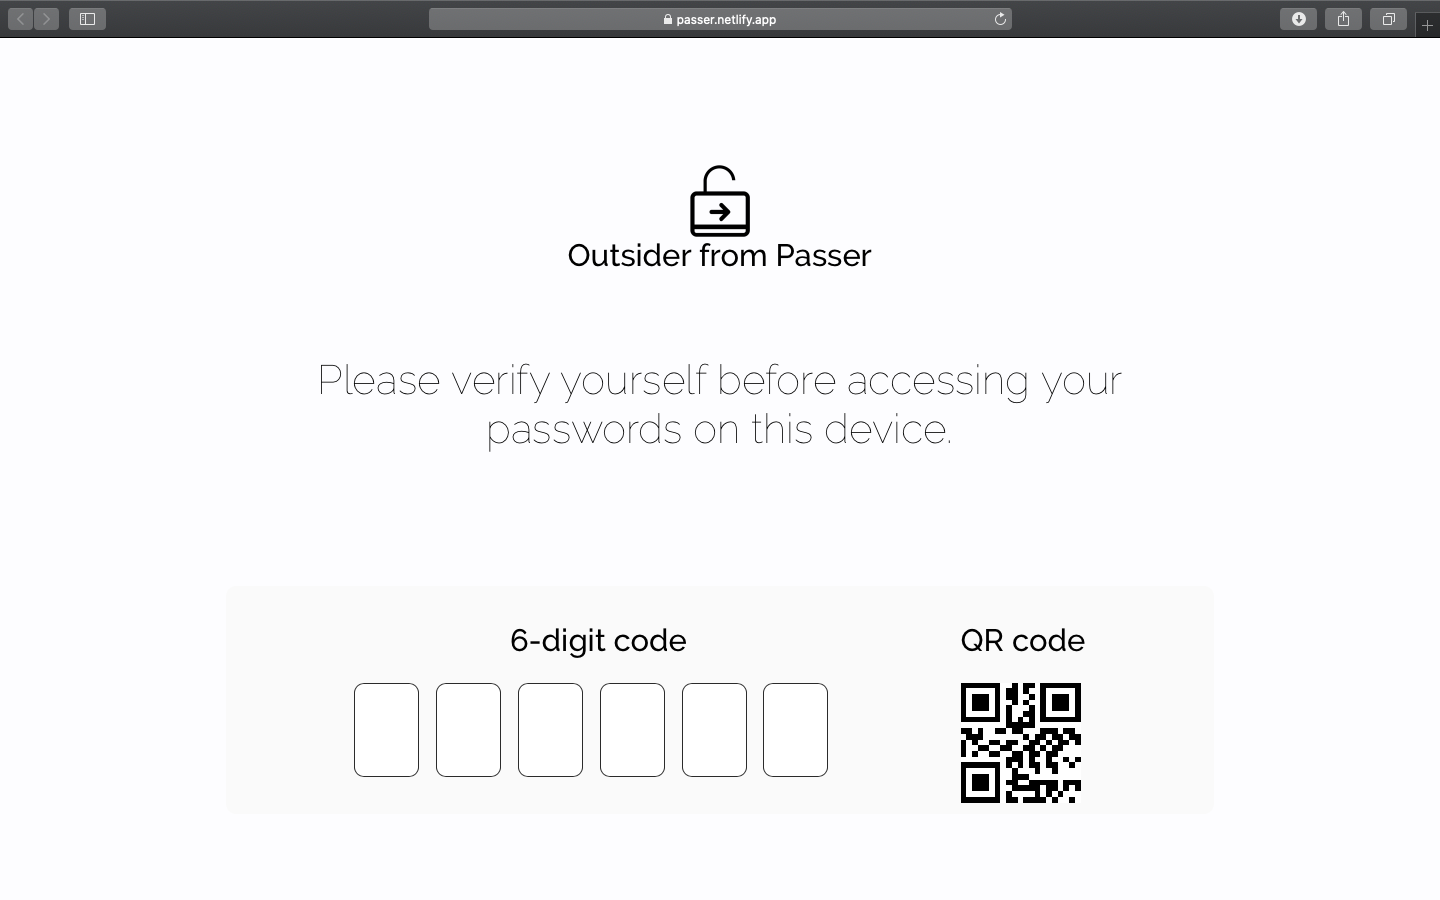
\includegraphics[width=15cm]{img/website1.png}
  \caption{Webstránka - Úvodná obrazovka.}
  \label{website1}
\end{figure}

\begin{figure}[H]
  \centering
  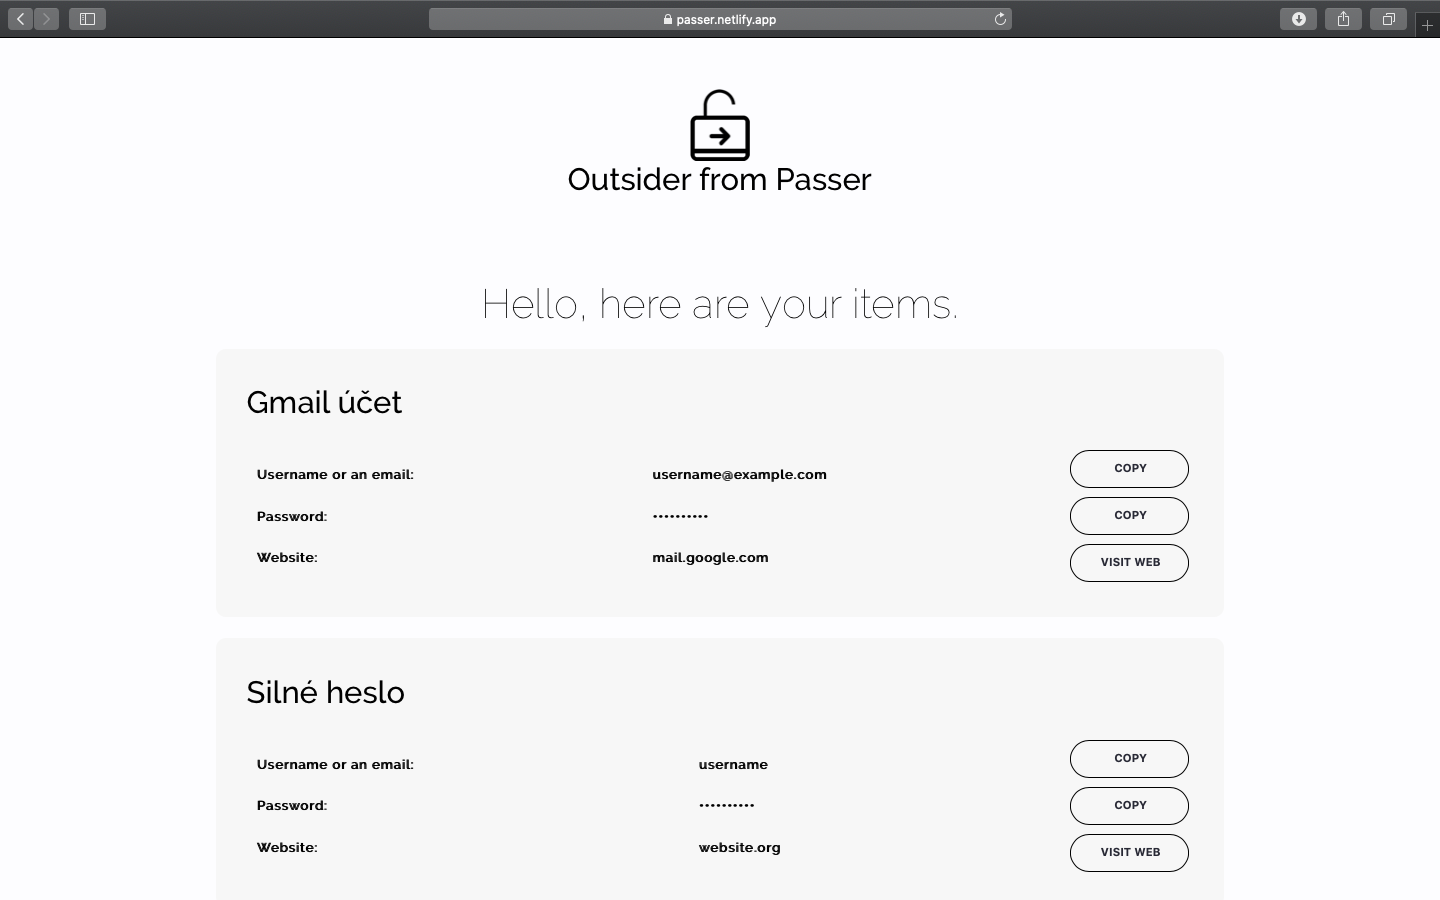
\includegraphics[width=15cm]{img/website2.png}
  \caption{Webstránka - Zobrazenie Passer položiek.}
  \label{website2}
\end{figure}